\documentclass[10pt]{beamer}

\usetheme[progressbar=frametitle]{metropolis}
\usepackage{appendixnumberbeamer}

\usepackage{booktabs}
\usepackage[scale=2]{ccicons}

\usepackage{pgfplots}
\usepgfplotslibrary{dateplot}

\usepackage{xspace}
\newcommand{\themename}{\textbf{\textsc{metropolis}}\xspace}

\usepackage{subcaption}
\usepackage{caption}

\usepackage{mathtools}
\usepackage[utf8]{inputenc}
\newcommand{\BK}[1]{ {\left( #1 \right)} }
\newcommand{\sqBK}[1]{ {\left[ #1 \right]} }
\newcommand{\curBK}[1]{ {\left\{ #1 \right\}} }
\newcommand{\bra}[1]{\langle #1 \rangle}
\newcommand{\p}[2]{\frac{\partial #1 }{\partial #2 }}
%\newcommand{\d}[2]{\frac{d #1 }{d #2 }}
\newcommand{\normal}[2]{\mathcal{N}( #1 , #2 )}
\newcommand{\R}{\mathbb{R}}
%\newcommand{\M}{\mathcal{M}}
\newcommand{\E}{\mathbb{E}}
\newcommand{\N}{\mathcal{N}}
\newcommand{\Q}{\mathbb{Q}}
\newcommand{\s}{\sigma}
%\newcommand{\T}{\text{T}}
\newcommand{\dFdw}{\frac{\partial F}{\partial w}}
\newcommand{\dFdu}{\frac{\partial F}{\partial u}}
\newcommand{\dwdu}{\frac{\partial w}{\partial u}}
\newcommand{\ddFdw}{\frac{\partial^2 F}{\partial w^2}}
\newcommand{\ddFdu}{\frac{\partial^2 F}{\partial u^2}}
\newcommand{\ddwdu}{\frac{\partial^2 w}{\partial u^2}}
%\newcommand{\m}{\mathbf}

\title{Constrained Hamiltonian Monte Carlo for PDE Inverse Problems}
%\subtitle{A modern beamer theme}
% \date{\today}
\date{}

\author{Au Khai Xiang \inst{1} \and Matthew Graham \inst{2} \and Alexandre Thiery \inst{2}}
\institute{\inst{1} NUS Graduate School for Integrative Sciences and Engineering,\\
                        National University of Singapore \and %
                      \inst{2} Department of Statistics and Applied Probability,\\
                      National University of Singapore}
% \titlegraphic{\hfill\includegraphics[height=1.5cm]{logo.pdf}}

\begin{document}
\maketitle

\begin{frame}{Table of contents}
  \setbeamertemplate{section in toc}[sections numbered]
  \tableofcontents[hideallsubsections]
\end{frame}

\section{Setup}

\begin{frame}[fragile]{Inverse Problem}

    Consider a data model with additive noise,
    
    $$y = F(z) + \sigma n. $$
    
    where\\
    $z \in \R^d$ is the latent variable\\
    $F: \R^d \rightarrow \R^m$ is the forward operator on $z$\\
    $n \sim \N(0, I_{m \times m}) \in \R^m$ is the noise variable\\
    $\s \in \R$ is noise intensity\\
    $y \in\R^m$ is the vector of data
    
    \begin{center}
    \alert{Given $y$, the task is to infer $z$.}
    \end{center}
  
\end{frame}

\begin{frame}[fragile]{From Model to Manifold}

    Standard approach: MCMC on the unconstrained latent space.

    Taking the $m$ observations to be constraints, we implicitly define a \alert{manifold}, $\mathcal{M}$ embedded in ambient space, $\R^{d+m}$.

    $$ \mathcal{M} = \{(z,n) \in \R^d \times \R^m: F(z) + \sigma n - y = 0\} $$
    
    \vspace{10pt}
    
    Alternate approach: MCMC on the \alert{constrained joint latent-noise space}.
    
\end{frame}

\begin{frame}[fragile]{Toy Model}

    Say we want to infer $z \in \R^2$. We are given
    $$F(z) = z_0^2 + z_1^2, \qquad \sigma \sim \N(0,1), \qquad \text{and} \qquad  y = 1.02.$$ 
    
    \vspace{20pt}
    
    Assuming $z\sim \N(0, I_{2 \times 2})$, we can write down the posterior.
    $$p(z|y) \propto \text{exp}\frac{-z^T z}{2} \, \text{exp}\frac{-(y - F(z))^2}{2 \sigma^2}   $$

\end{frame}

\begin{frame}[fragile]{The Low-Noise Regime (Latent Space)}
    
    As $\sigma$ tends to 0, posterior mass concentrates in the neighbourhood of the manifold, $M_{\sigma=0} =\{z : F(z) = y\}$.
    
    \begin{figure}
        \begin{subfigure}[b]{0.3\textwidth}
            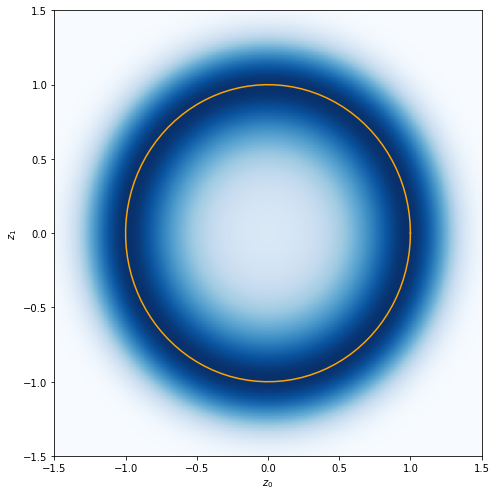
\includegraphics[width=\textwidth]{manifold_high_noise.png}
            \subcaption{$\sigma = 0.5$}
        \end{subfigure}%
        \begin{subfigure}[b]{0.3\textwidth}
            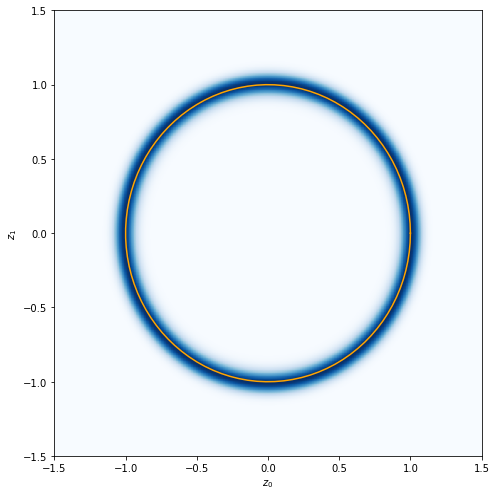
\includegraphics[width=\textwidth]{manifold_mid_noise.png}
            \subcaption{$\sigma = 0.1$}
        \end{subfigure}%
        \begin{subfigure}[b]{0.3\textwidth}
            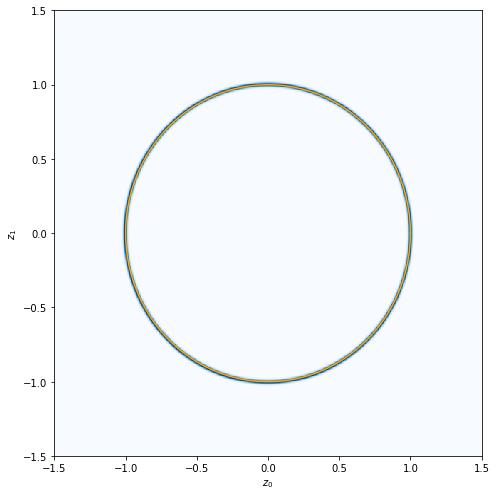
\includegraphics[width=\textwidth]{manifold_low_noise.png}
            \subcaption{$\sigma = 0.02$}
        \end{subfigure}
        \caption{Visualisations of posterior densities with decreasing noise}
    \end{figure}
   
    ...MCMC may only take \alert{small step-sizes.}
    
\end{frame}

\begin{frame}[fragile]{The Low-Noise Regime (Joint Latent-Noise Space)}

    By lifting the problem into the joint latent-noise space, MCMC may take \alert{larger step-sizes} on the manifold.


    \begin{figure}
        \begin{subfigure}[b]{0.32\textwidth}
            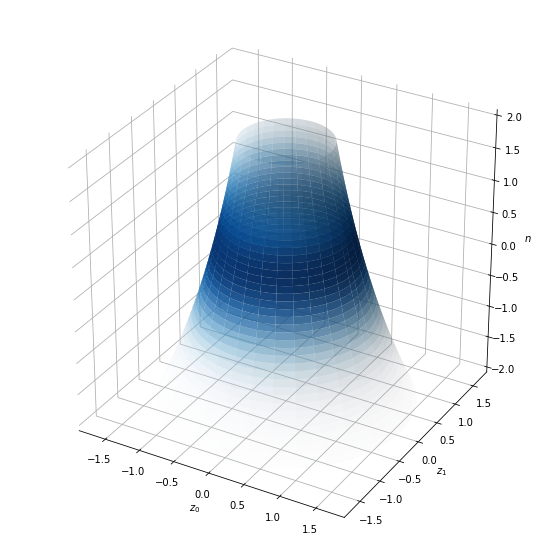
\includegraphics[width=\textwidth]{m_high_noise.png}
            \subcaption{$\sigma = 0.5$}
        \end{subfigure}%
        \begin{subfigure}[b]{0.32\textwidth}
            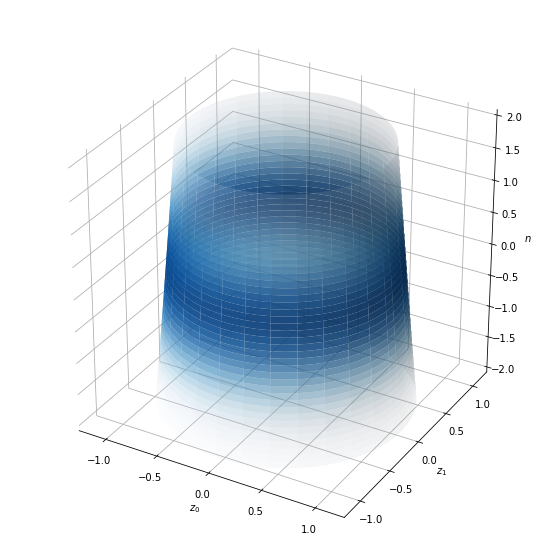
\includegraphics[width=\textwidth]{m_mid_noise.png}
            \subcaption{$\sigma = 0.1$}
        \end{subfigure}%
        \begin{subfigure}[b]{0.32\textwidth}
            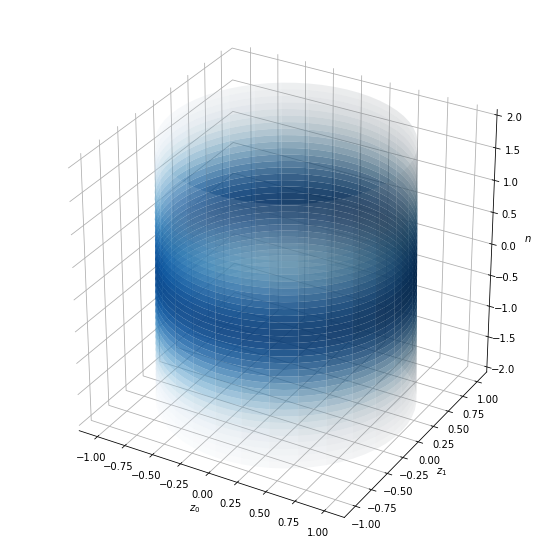
\includegraphics[width=\textwidth]{m_low_noise.png}
            \subcaption{$\sigma = 0.02$}
        \end{subfigure}
        \caption{Visualisations of manifold with decreasing noise}
    \end{figure}
    
\end{frame}

\section{Constrained HMC Method}

\begin{frame}[fragile]{Refresher on HMC}
    To infer $z$, we need
    \begin{itemize}
        \item Posterior distribution, $p(z|y) \propto p(y|z) \,\pi(z)$ 
        \item Potential energy, $U(z) = -\text{log }p(z|y)$.
        \item Gradient of potential energy, $\frac{dU(z)}{dz}$
    \end{itemize}
    \vspace{10pt}
    Throughout, we assume an isotropic Gaussian momentum variable.
\end{frame}

\begin{frame}[fragile]{Constrained HMC setup}
    Joint variable and constraint function
    $$q \coloneqq [z, n], \qquad \qquad c(q) = F(z) + \sigma n - y = 0$$
    
    Jacobian of constraint
    $$J(q) = \Big[ \p{c}{z} \p{c}{n} \Big] = \Big[ \frac{dF}{dz} \quad \sigma I_{m \times m} \Big] $$
    
    Distribution on manifold
    $$\pi_\mathcal{M}(q) = \pi(q) |J(q) \, J(q) ^T|^{-1/2}$$
\end{frame}

\begin{frame}[fragile]{Constrained HMC setup}
    Potential Energy
    \begin{align*}
    U(q) = -\text{log }\pi_\mathcal{M}(q) &= -\text{log }\pi(q) + \frac{1}{2}\text{log } |J(q) \, J(q)^T| \\
    &= -\text{log }\pi(q) + \frac{1}{2} \text{log }\Bigg| \frac{dF}{dz} \frac{dF}{dz}^T  + \sigma^2 I\Bigg| \\
    &= Z + \frac{q^T q}{2} + \sum_i \text{log } L_{ii}\\
    \end{align*}
    
    (Part of) Gradient of Potential Energy
    $$\frac{d}{dz} \Big( \frac{1}{2} \text{log }\Big| \frac{dF}{dz} \frac{dF}{dz}^T  + \sigma^2 I\Big| \Big) = \text{Tr} \Bigg(  \Big( \frac{dF}{dz} \frac{dF}{dz}^T + \sigma^2 I\Big)^{-1}\frac{dF}{dz} \frac{\partial^2 F^T}{\partial z_i \partial z} \Bigg)$$

\end{frame}

\begin{frame}[fragile]{RATTLE Algorithm}

One step in a trajectory
\begin{align*}
    p_{1/2} &= p_0 - \frac{h}{2}(\nabla U(q_0) + J(q_0)^T \lambda)\\
    q_1 &= q_0 + h \, p_{1/2}\\
    0 &= c(q_1)\\
    p_1 &= p_{1/2} - \frac{h}{2}(\nabla U(q_1) + J(q_1)^T \mu)\\
    0 &= J(q_1) \, p_1
\end{align*}

Unconstrained update of $q$, project onto $M$.\\
Unconstrained update of $p$, project onto tangent space of $M$.

\end{frame}


\begin{frame}[fragile]{Inferring on $z$}

    \begin{figure}
        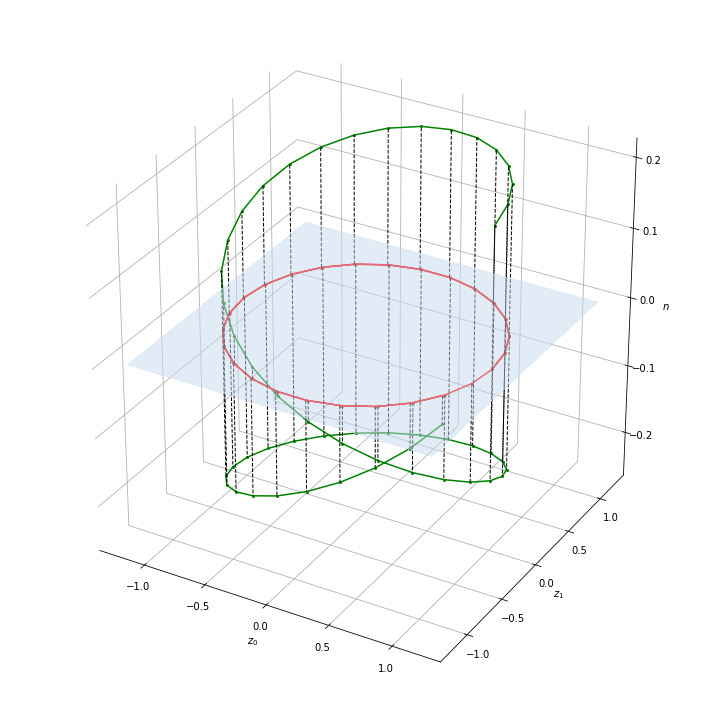
\includegraphics[width=0.5\textwidth]{traj_0.1.png}
        \caption{Trajectory with projection onto latent space}
    \end{figure}
    
    With samples of $q$, we can then simply drop the noise components $n$ and just retain $z$.

\end{frame}

\begin{frame}[fragile]{Position and Momentum Projections}
    (Non-linear) Position Projection - e.g. Quasi-Newton method

    $$ \text{while } \Vert c(q) \Vert_\infty > \text{tol}: 
    q \leftarrow q - J_q^T ( J_q \, J_q^T)^{-1} c(q)$$ 
    
    (Linear) Momentum Projection
	$$ p \leftarrow p - J_q^T ( J_q \, J_q^T)^{-1} J_q \, p$$
	
	\alert{As such, $q$ stays on the manifold while $p$ stays in the tangent space of the manifold at $q$.}

\end{frame}

\begin{frame}[fragile]{Effects of Step Size on the RATTLE Scheme}

    \begin{figure}
        \begin{subfigure}[b]{0.32\textwidth}
            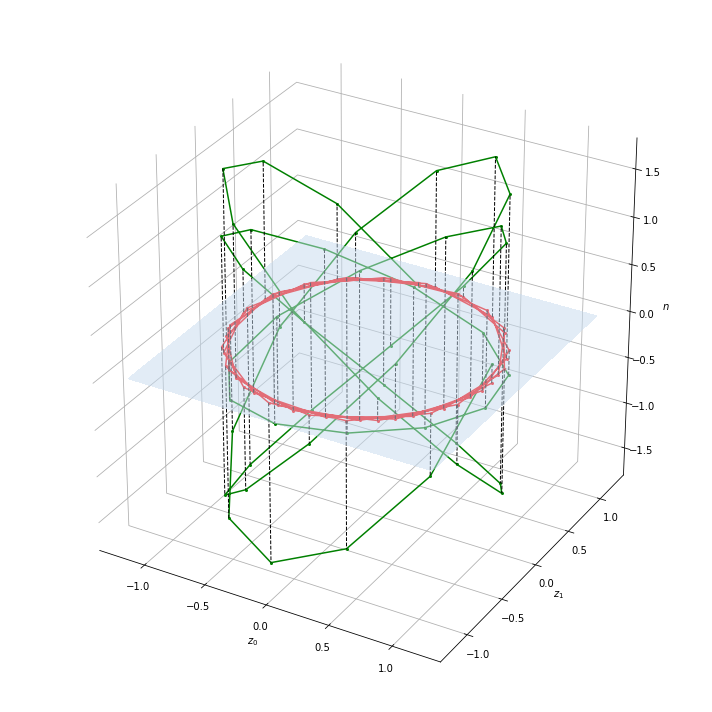
\includegraphics[width=\textwidth]{traj_0.5.png}
            \subcaption{step size = 0.5}
        \end{subfigure}%
        \begin{subfigure}[b]{0.32\textwidth}
            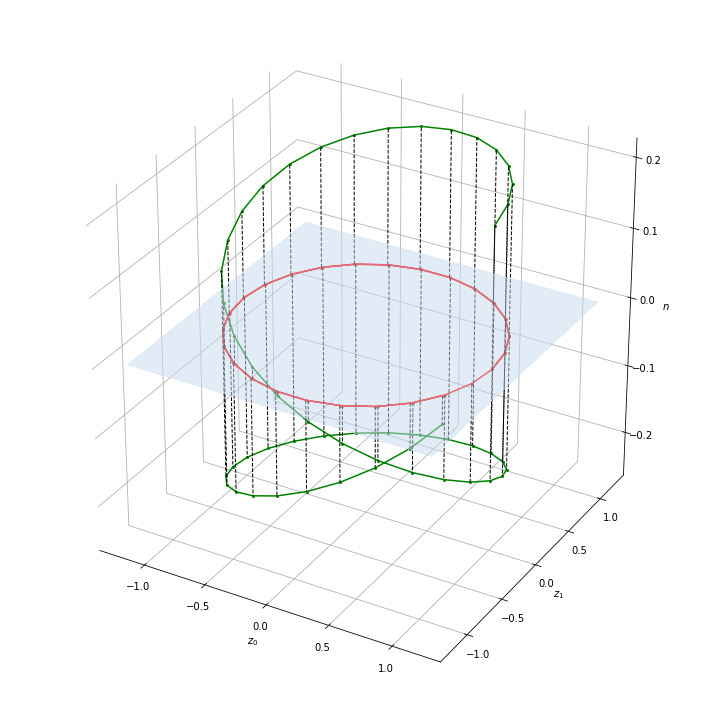
\includegraphics[width=\textwidth]{traj_0.1.png}
            \subcaption{step size = 0.1}
        \end{subfigure}%
        \begin{subfigure}[b]{0.32\textwidth}
            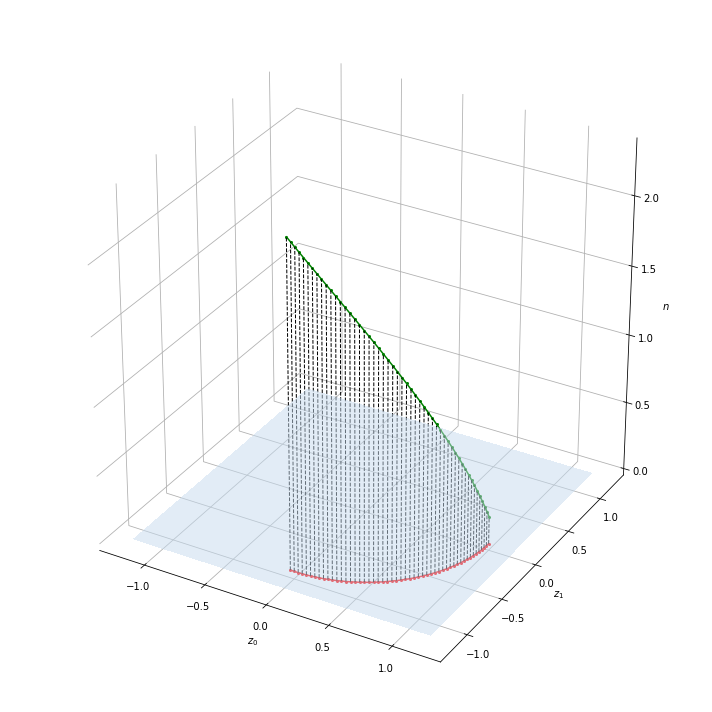
\includegraphics[width=\textwidth]{traj_0.02.png}
            \subcaption{step size = 0.02}
        \end{subfigure}
        \caption{Constrained HMC trajectory and projections onto latent space}
    \end{figure}

\end{frame}


\begin{frame}{Maintaining reversibility}
    On top of the usual Metropolis-Hastings scheme, we uphold reversibility by rejecting a sample when
    \begin{itemize}
        \item Quasi-Newton method fails to converge
        \item A reverse RATTLE step fails to return its previous point in phase space.
    \end{itemize}
    
    Note: this is consistent with any choice of tolerance for the Quasi-Newton method.
\end{frame}

\begin{frame}[fragile]{Implementation Details}

    At every new $q$:
    \begin{itemize}
        \item Compute and store Jacobian, $J(q)$.
        \item (Sparse) Cholesky decomposition on gram matrix, $$LL^T = J(q) \, J(q)^T.$$
        \item Compute hessian of $F(z)$ for $\nabla U(q)$.
    \end{itemize}
    
    \vspace{10pt}
    For reverse step checks, Jacobian matrices are stored and reused.
    
    $$q_0 \xrightleftharpoons[J(q_1)]{J(q_0)} q_1 \xrightleftharpoons[J(q_2)]{J(q_1)} q_2 \xrightleftharpoons[J(q_3)]{J(q_2)} \dots$$
    
\end{frame}

\section{Results}

\begin{frame}[fragile]{Visual Comparison for Sampling Efficiency}
       \begin{figure}
       
        \begin{subfigure}[b]{0.42\textwidth}
            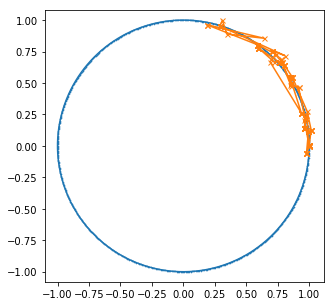
\includegraphics[width=\textwidth]{v_samples.png}
            \subcaption{HMC samples}
        \end{subfigure}%
        \qquad \qquad
        \begin{subfigure}[b]{0.42\textwidth}
            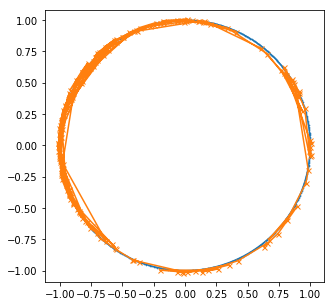
\includegraphics[width=\textwidth]{samples.png}
            \subcaption{Constrained HMC samples}
        \end{subfigure}
        \caption{MCMC chain of 200 samples, step size = 0.005, noise intensity = 0.02}
    \end{figure}
\end{frame}

\begin{frame}[fragile]{Exploring the Target Distribution}
        \begin{figure}
                \centering
                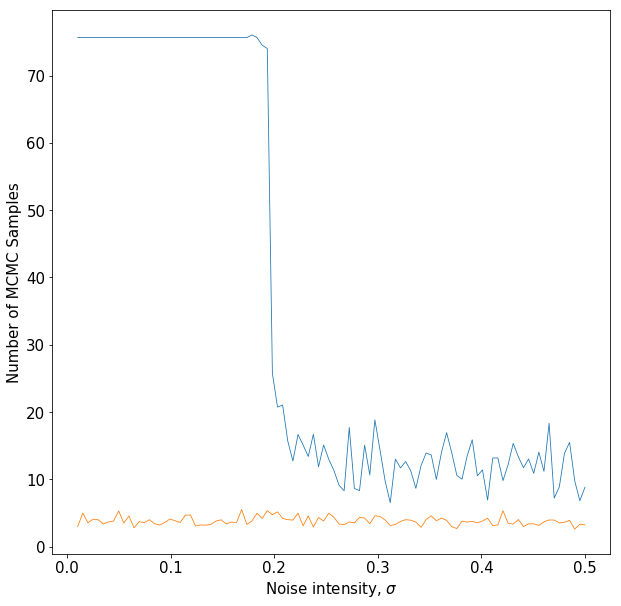
\includegraphics[width=0.6\textwidth]{iters_vs_noise.png}
                \caption{Iterations taken to explore left half of the target distribution}
        \end{figure}
\end{frame}

\begin{frame}[fragile]{Exploring the Target Distribution}
        \begin{figure}
            \centering
            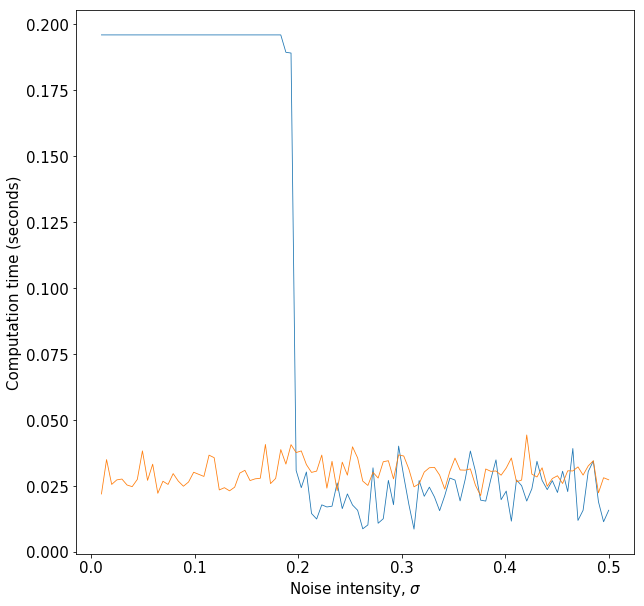
\includegraphics[width=0.6\textwidth]{time_vs_noise.png}
            \caption{Time taken (seconds) to explore left half of the target distribution}
        \end{figure}
\end{frame}

\begin{frame}[fragile]{Mean Acceptance Probability}
    \begin{figure}
    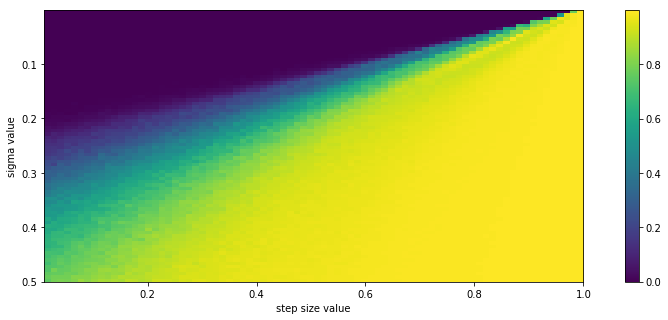
\includegraphics[width=\textwidth]{exp2.png}
    \caption{Heat map of mean acceptance probability}
    \end{figure}
\end{frame}

\begin{frame}[fragile]{Mean Acceptance Probability}
    [insert figure for constrained HMC]
\end{frame}

\begin{frame}[fragile]{PDE Inverse Problem}

    Consider a 2D non-linear Poisson's equation.

    $$ \nabla \cdot ( e^c \nabla u) = f$$
    
    where\\
    $c: \R^2 \rightarrow \R$  is the log coefficient field\\
    $f: \R^2 \rightarrow \R$ is the source term\\
    $u:  \R^2 \rightarrow \R$ is the solution of the PDE\\
    
    Task: With known $f$ and few noisy observations of $u$, infer $c$.
    
\end{frame}


\begin{frame}[fragile]{PDE Inverse Problem}
     
    \begin{figure}
        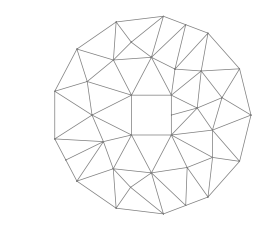
\includegraphics[width=0.5\textwidth]{pde_domain.png}
        \caption{2D domain mesh}
    \end{figure}
    
    Using the finite element method, our discretized PDE has dimensionality $d = 37$.
    
\end{frame}

\begin{frame}[fragile]{PDE Inverse Problem}
    
    We generate noisy observations of the solution field. With $m = 5$ observations (hence $m$ noise components), our inverse problem is of size $d + m $.
    
       \begin{figure}
        \begin{subfigure}[b]{0.21\textwidth}
            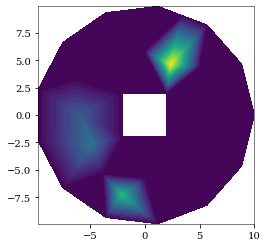
\includegraphics[width=\textwidth]{pde_obs.png}
            \subcaption{5 solution observations}
        \end{subfigure}%
        \qquad \qquad \qquad
        \begin{subfigure}[b]{0.42\textwidth}
            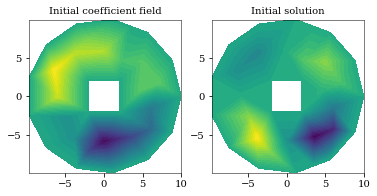
\includegraphics[width=\textwidth]{pde_initial.png}
            \subcaption{Initial coefficient and solution}
        \end{subfigure}
        \caption{PDE inverse problem setup}
    \end{figure}
\end{frame}

\begin{frame}[fragile]{PDE Inverse Problem}
       \begin{figure}
       
        \begin{subfigure}[b]{0.42\textwidth}
            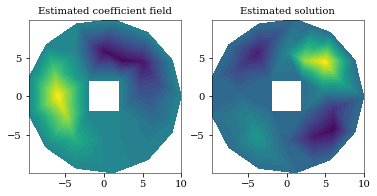
\includegraphics[width=\textwidth]{pde_estimate.png}
            \subcaption{Ground truth coefficient and solution}
        \end{subfigure}%
        \qquad \qquad
        \begin{subfigure}[b]{0.42\textwidth}
            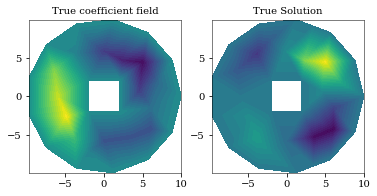
\includegraphics[width=\textwidth]{pde_true.png}
            \subcaption{Estimated coefficient and solution}
        \end{subfigure}
        \caption{Constrained HMC results}
    \end{figure}
\end{frame}

\begin{frame}{References}
  Some references to showcase [allowframebreaks] \cite{knuth92,ConcreteMath,Simpson,Er01,greenwade93}
\end{frame}

\section{Conclusion}
\begin{frame}[fragile]
The data model informs a manifold on which MCMC sampling is more efficient than on the unconstrained posterior.

The efficiency of constrained HMC outweighs its computation costs when we have precise measurements.
\end{frame}

% \appendix

\begin{frame}[allowframebreaks]{References}

  \bibliography{demo}
  \bibliographystyle{abbrv}

\end{frame}

\end{document}